% !TEX root = ../my-thesis.tex
%
\chapter{Status of dark matter searches with ATLAS}
\label{sec:outlook}

\section{Introduction}
\label{sec:outlook:intro}
This chapter relates the results presented in this dissertation to the broader picture and aims to provide an overview of the experimental status of ATLAS mediator-based dark matter searches.

The public ATLAS results based on the \HepProcess{\Pp\Pp} collision data collected in the Run-2 data-taking during 2015--2018 are summarised in the context provided by models for dark matter production. As no significant excess over the expected SM background was observed in any of these searches, constraints on the parameter space of three classes of dark matter models are presented.

\Cref{sec:outlook:dmsimp} discusses limits on simplified models with spin-1 \PZprime mediators.
\Cref{sec:outlook:higgs} discusses the limits on simplified models with extended Higgs sector. Finally, \Cref{sec:outlook:2mdm} discusses the limits on simplified models with two mediators.

\section{Simplified models with spin-1 \PZprime mediators}
\label{sec:outlook:dmsimp}
The \(V/A\) simplified model (c.f. ~\Cref{sec:dm:models:dmsimp}) is strongly constrained by searches for the associated production of dark matter particles with ISR objects and by searches for high-mass resonances decaying into pairs of fermions. The resonance searches can place limits on the \(V/A\) simplified model, as the production of dark matter via a mediator produced from quarks also establishes the inverse process of the mediator decaying to quarks. Therefore, these limits have very little dependence on \mchi and can exclude large regions of parameter space.

\Cref{fig:outlook:dmsimp:vector-axial} shows the constraints on the \PZprime boson vector and axial-vector mediator scenarios for the parameters \(\gq = 0.25\), \(\gl = 0\), \(\gchi = 1\) in the \mZp-\mchi plane.

\begin{figure}[htbp]
    \centering
    \begin{subfigure}{1.\textwidth}
    \centering
    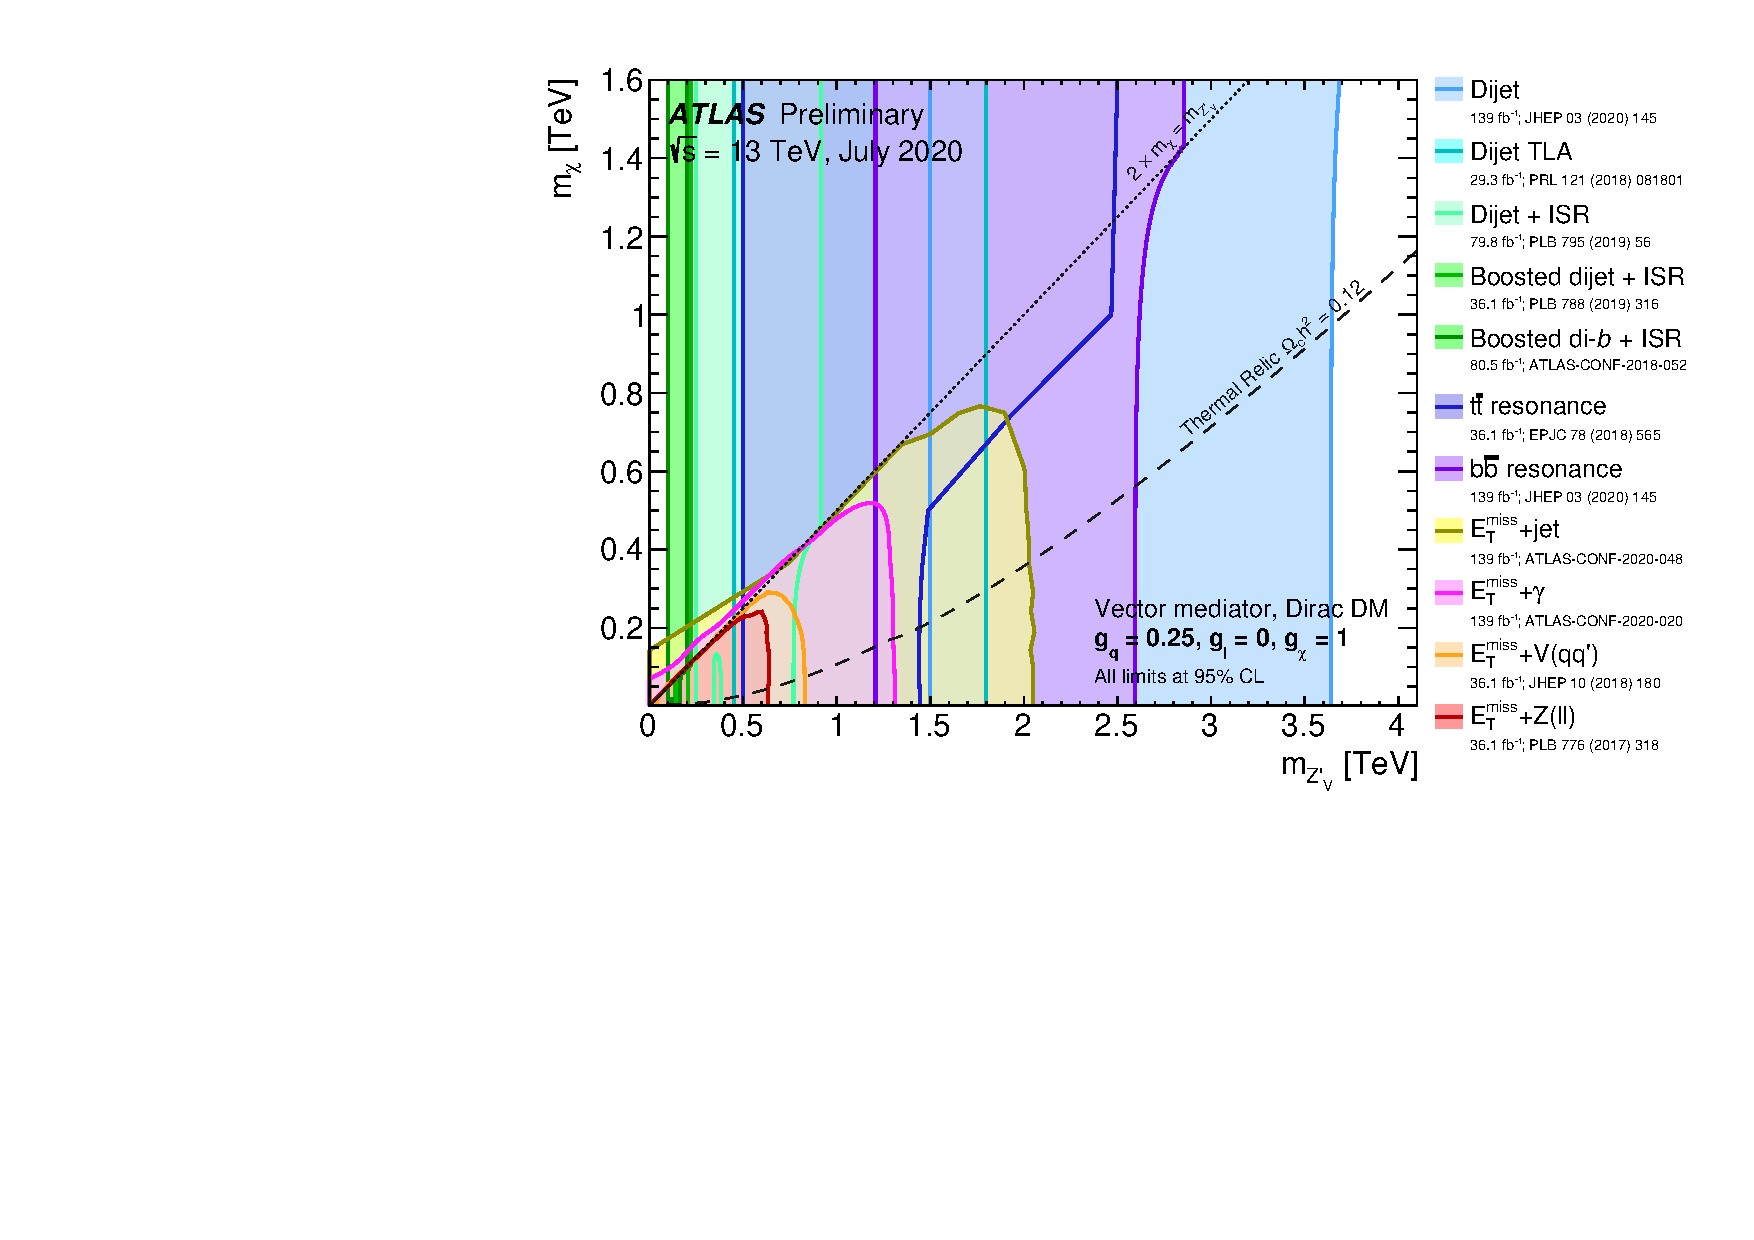
\includegraphics[width=1.\textwidth]{figures/outlook/dmsimp/dmsimp-vector.pdf}
    \caption{Vector mediator}
  \end{subfigure}
  \\
  \begin{subfigure}{1.\textwidth}
    \centering
    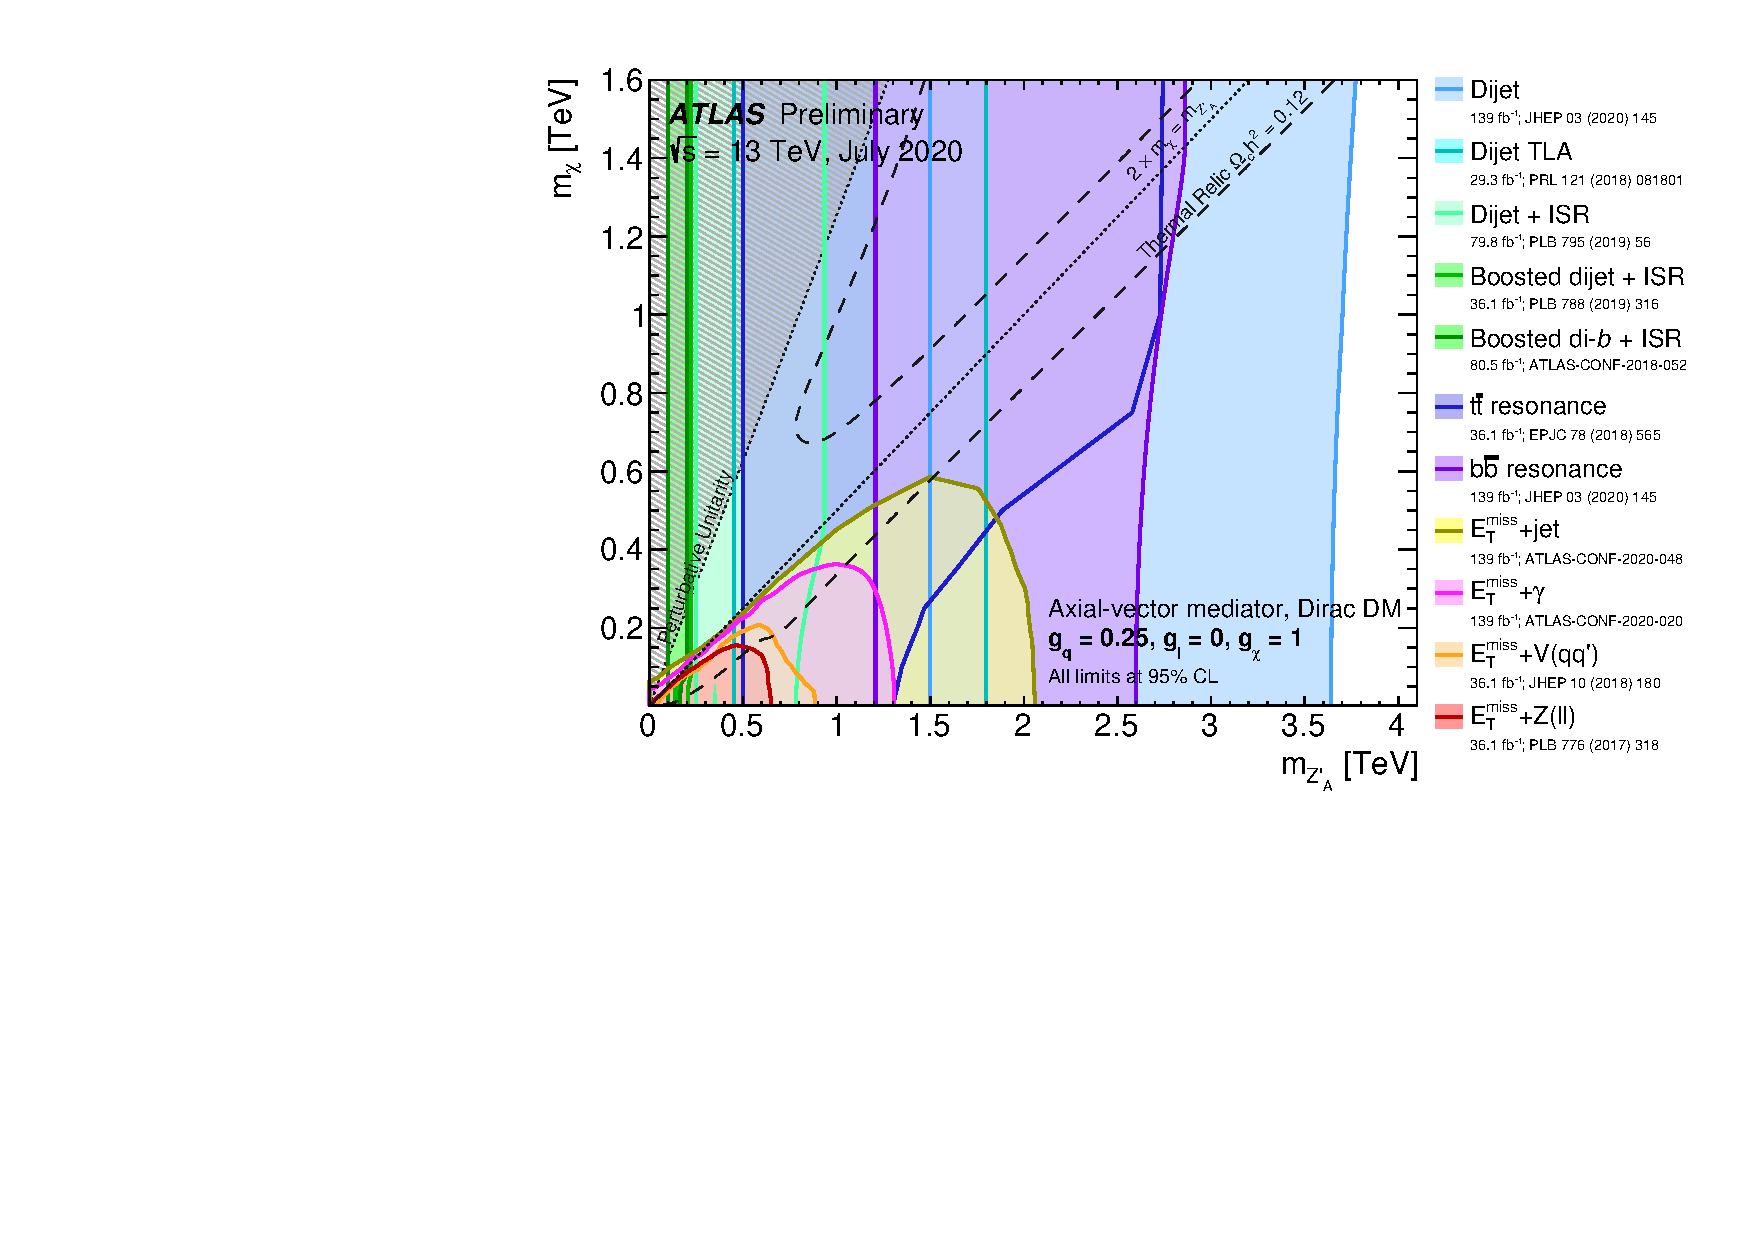
\includegraphics[width=1.\textwidth]{figures/outlook/dmsimp/dmsimp-axial.pdf}
    \caption{Axial-vector mediator}
  \end{subfigure}
    \caption{Regions in the \mZp-\mchi plane in the parameter space of the spin-1 \PZprime mediator simplified model excluded at \SI{95}{\percent} \(\text{CL}_{s}\) for the choice of vector (top) and axial-vector (bottom) mediator mediator couplings \(\gq = 0.25\), \(\gchi = 1\), \(\gl = 0\). The dashed curve indicates combinations of mediator mass \mZp and dark matter particle mass \mchi which are consistent with the Planck~\cite{Planck2020} dark matter relic density  measurements. The dotted line indicates the kinematic threshold where the mediator can decay on-shell into dark matter particles. The shading in the upper left corner indicates regions which are in tension with perturbative unitary considerations. Figures reproduced from Ref.~\cite{ATL-PHYS-PUB-2020-021}.}
    \label{fig:outlook:dmsimp:vector-axial}
\end{figure}

The combinations of \mZp and \mchi, which result in the observed relic density \(\Omega h^2 = 0.12\) from Planck~\cite{Planck2020} measurements are indicated by dashed curves labelled with \emph{thermal relic}. The kinematic threshold where on-shell decays of the mediator to dark matter particles become possible is indicated by a dotted line.
Also, the regions which are in tension with considerations of perturbative unitarity~\cite{Kahlhoefer2016} are indicated by shading.

The most stringent limits for the chosen benchmark scenario with \(\gq = 0.25\) are placed by the dijet search, with exclusion up to \(\mZp = \SI{3.6}{\tera\electronvolt}\). Its lower mass reach down to \SI{460}{\giga\electronvolt} is limited by the jet trigger threshold. Therefore, two alternative search strategies are employed to circumvent this limitation. The trigger-level-analysis (TLA) stores event information at trigger-level with reduced detector information to allow for a lower mass threshold. The searches in the dijet + ISR family trigger on additional ISR objects and can therefore set limits on mediator masses as low as \SI{100}{\giga\electronvolt}. In addition, the searches for di-\bjet and top quark pair resonances place complementary exclusion limits.

The \(\met + X\) family of searches are most sensitive in the on-shell region \(2 \mchi < \mZp\).
Their sensitivity decreases in the off-shell region due to a strong decrease in the production cross-section. Therefore, only the \(\met + \text{jet}\) and \(\met + \Pgamma\) searches can probe this region and only for low \mZp and \mchi.
In addition to the limit of the \(\met + \Vqq\) search, the results of the  \(\met + \HepProcess{\PZ(\Pl\Pl)}\) search is shown, which is also based on \SI{36.1}{\per\femto\barn} \HepProcess{\Pp\Pp} collision data. The \(\met + \Vqq\) search is more sensitive than the \(\met + \HepProcess{\PZ(\Pl\Pl)}\) search because it targets both \PW and \PZ weak vector bosons and because of the larger weak vector boson branching fraction to hadronic decays.
The \(\met + \Pgamma\) search is based on the full Run-2 dataset and benefits from the larger production cross-section of photon ISR. Therefore, the reach of the exclusion extends up to \SI{1.3}{\tera\electronvolt}, which is more than twice the reach of the \(\met + \Vqq\) search.
The largest exclusion of up to \SI{2.0}{\tera\electronvolt} in \mZp and \SI{750}{\giga\electronvolt} in \mchi is provided by the \(\met + \text{jet}\) search, which benefits also from the full Run-2 dataset and from the largest production cross-section.

Large regions of the viable parameter space for the \(V/A\) simplified model are ruled out for the mediator couplings under consideration. However, alternative coupling scenarios correspond to different regions of excluded parameter space. A reduced coupling of the mediator to quarks results in smaller reach of the dijet searches and gives more emphasis to the \(\met + X\) limits, thereby demonstrating the interplay of the two approaches.

Collider experiments provide a complementary approach to direct and in-direct detection experiments (c.f. \Cref{sec:dm:searches}).
The \(V/A\) simplified model allows comparing the collider-based limits with those of direct detection experiments.
\Cref{fig:outlook:dmsimp:dd} shows the limits on the spin-independent \(\chi\)-nucleon scattering cross-sections as a function of the dark matter mass \mchi.

\begin{figure}[htbp]
    \centering
    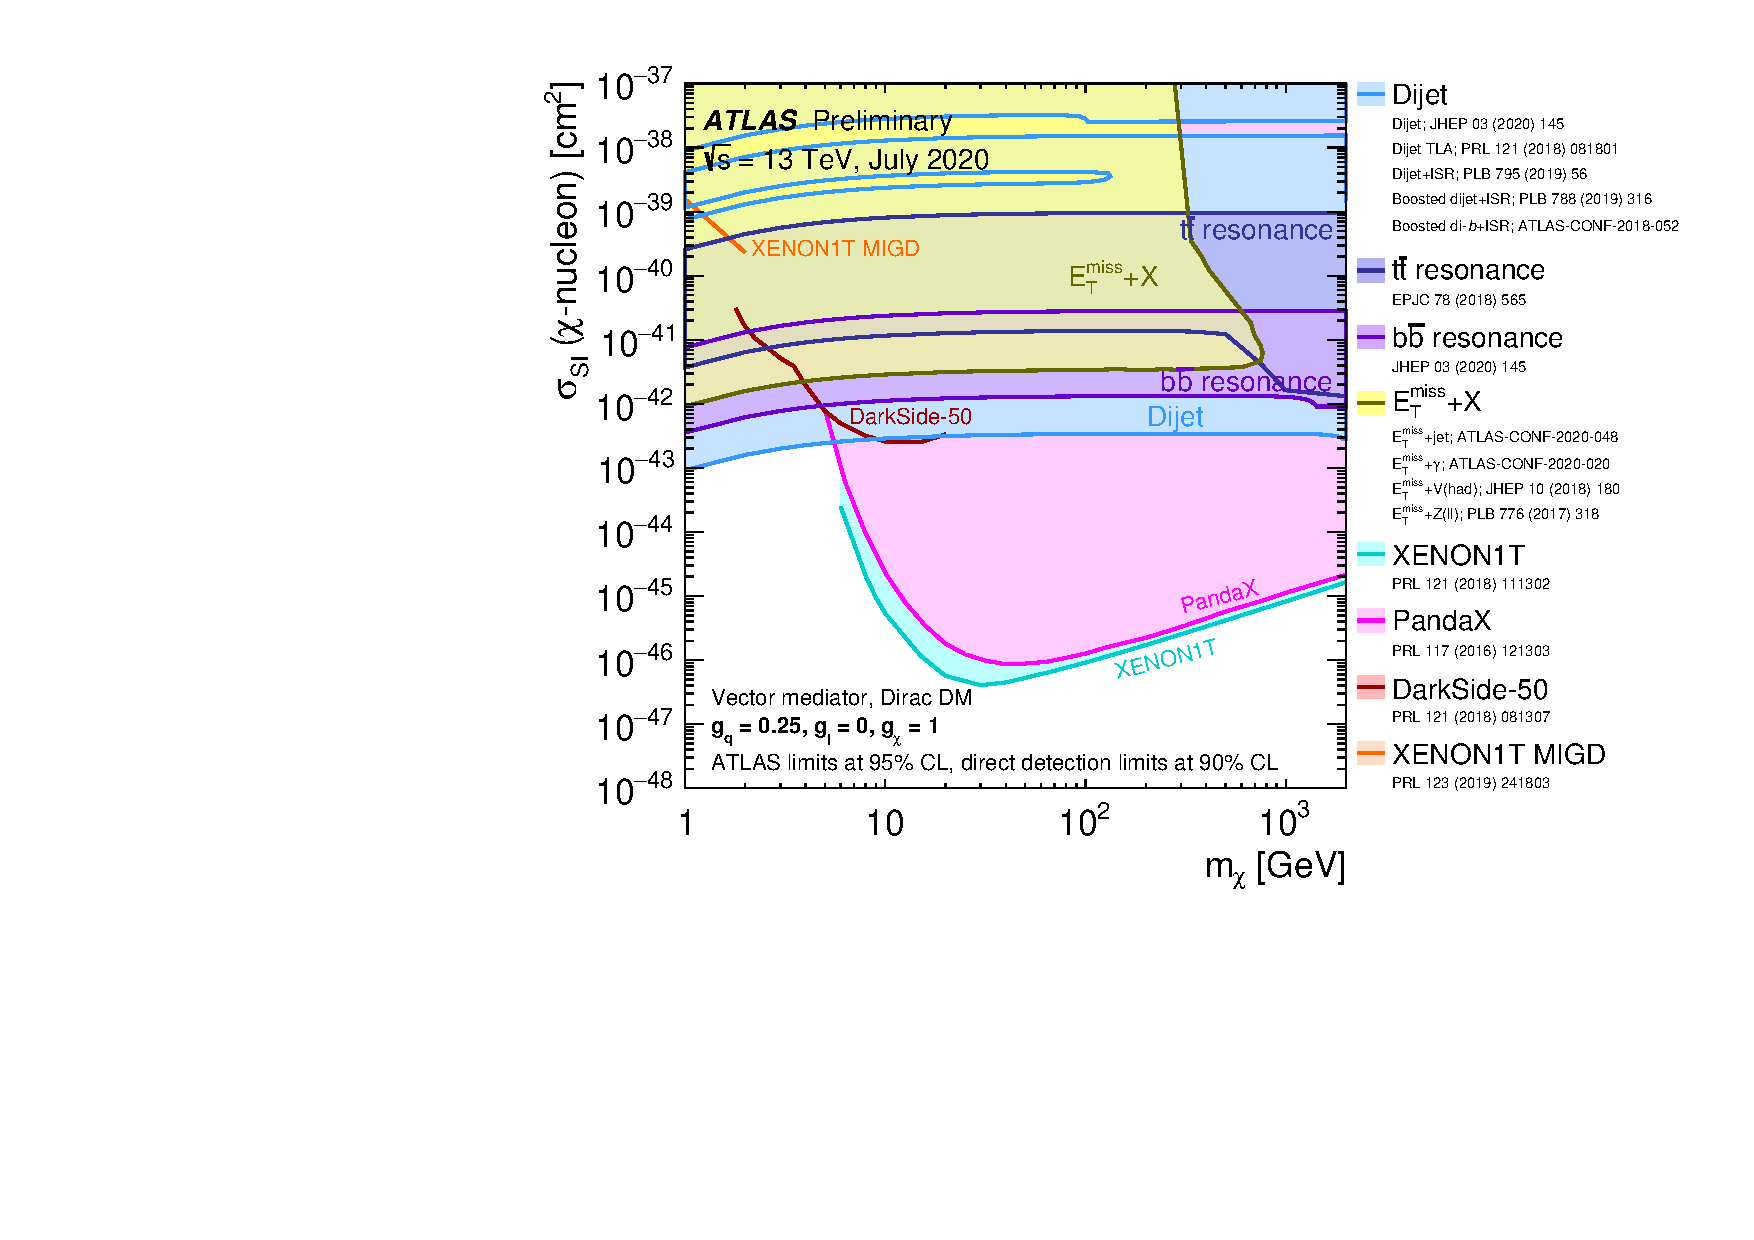
\includegraphics[width=1.\textwidth]{figures/outlook/dmsimp/dmsimp-DD-vectorpdf.pdf}
    \caption{Regions in the \mZp-\mchi plane in the parameter space of the spin-1 \PZprime axial-vector mediator simplified model excluded at \SI{95}{\percent} \(\text{CL}_{s}\) for the choice of mediator couplings \(\gq = 0.25\), \(\gchi = 1\), \(\gl = 0\). The dashed curve indicates combinations of mediator mass \mZp and dark matter particle mass \mchi which are consistent with the Planck~\cite{Planck2020} dark matter relic density  measurements. The dotted line indicates the kinematic threshold where the mediator can decay on-shell into dark matter particles. The shaded region in the upper left corner indicates combinations of mediator mass \mZp and dark matter particle mass \mchi which are in tension with the perturbative unitary considerations. Figure reproduced from Ref.~\cite{ATL-PHYS-PUB-2020-021}.}
    \label{fig:outlook:dmsimp:dd}
\end{figure}

The direct detection experiments dominate the sensitivity by a few orders of magnitude for \(\mchi > \SI{6}{\giga\electronvolt}\). In the low \mchi range, the direct detection experiments have reduced sensitivity due to the very low energy recoil that light dark dark matter particles would induce. In this region, the resonance searches complement the direct detection limits.


\section{Simplified models with extended Higgs sector}
\label{sec:outlook:higgs}
Two models with an extended Higgs sector are considered in this dissertation. These models are the simplest extensions of the simplified models describing only dark matter particles and mediators. They address some of the shortcomings of these elementary simplified models, such as lacking the ingredients of UV-complete theories and consequently missing signatures which are contained in the broader phenomenology of more sophisticated models~\cite{Kahlhoefer2016}.

The \zhdm model, which is probed by the \(\met + \Hbb\) search, is strongly constrained by dijet searches and is subjected to additional indirect constraints from flavour-physics~\cite{Hermann2012,Misiak2015} and electro-weak precision measurements~\cite{Berlin2014}, leaving very little viable parameter space. Therefore, the following discussion is focused on the \ahdm simplified model (c.f. ~\Cref{sec:dm:models:ahdm}).

The \ahdm simplified model describes the interaction between SM particles and dark matter particles which is mediated by a pseudo-scalar mediator. Consequentially, not only the constraints from most resonance searches but also from direct-detection experiments are avoided. Therefore, collider-based searches are particularly important to test this class of models.

\Cref{fig:outlook:higgs:ahdm-mHma} shows the exclusion contours at at \SI{95}{\percent} \(\text{CL}_{s}\) in the \mA-\ma plane of the parameter space for the fixed choice of parameters \(\tan{\beta} = 1.0\), \(\mchi = \SI{10}{\giga\electronvolt}\), and \(\sin \theta = 0.35\).

\begin{figure}[htbp]
    \centering
    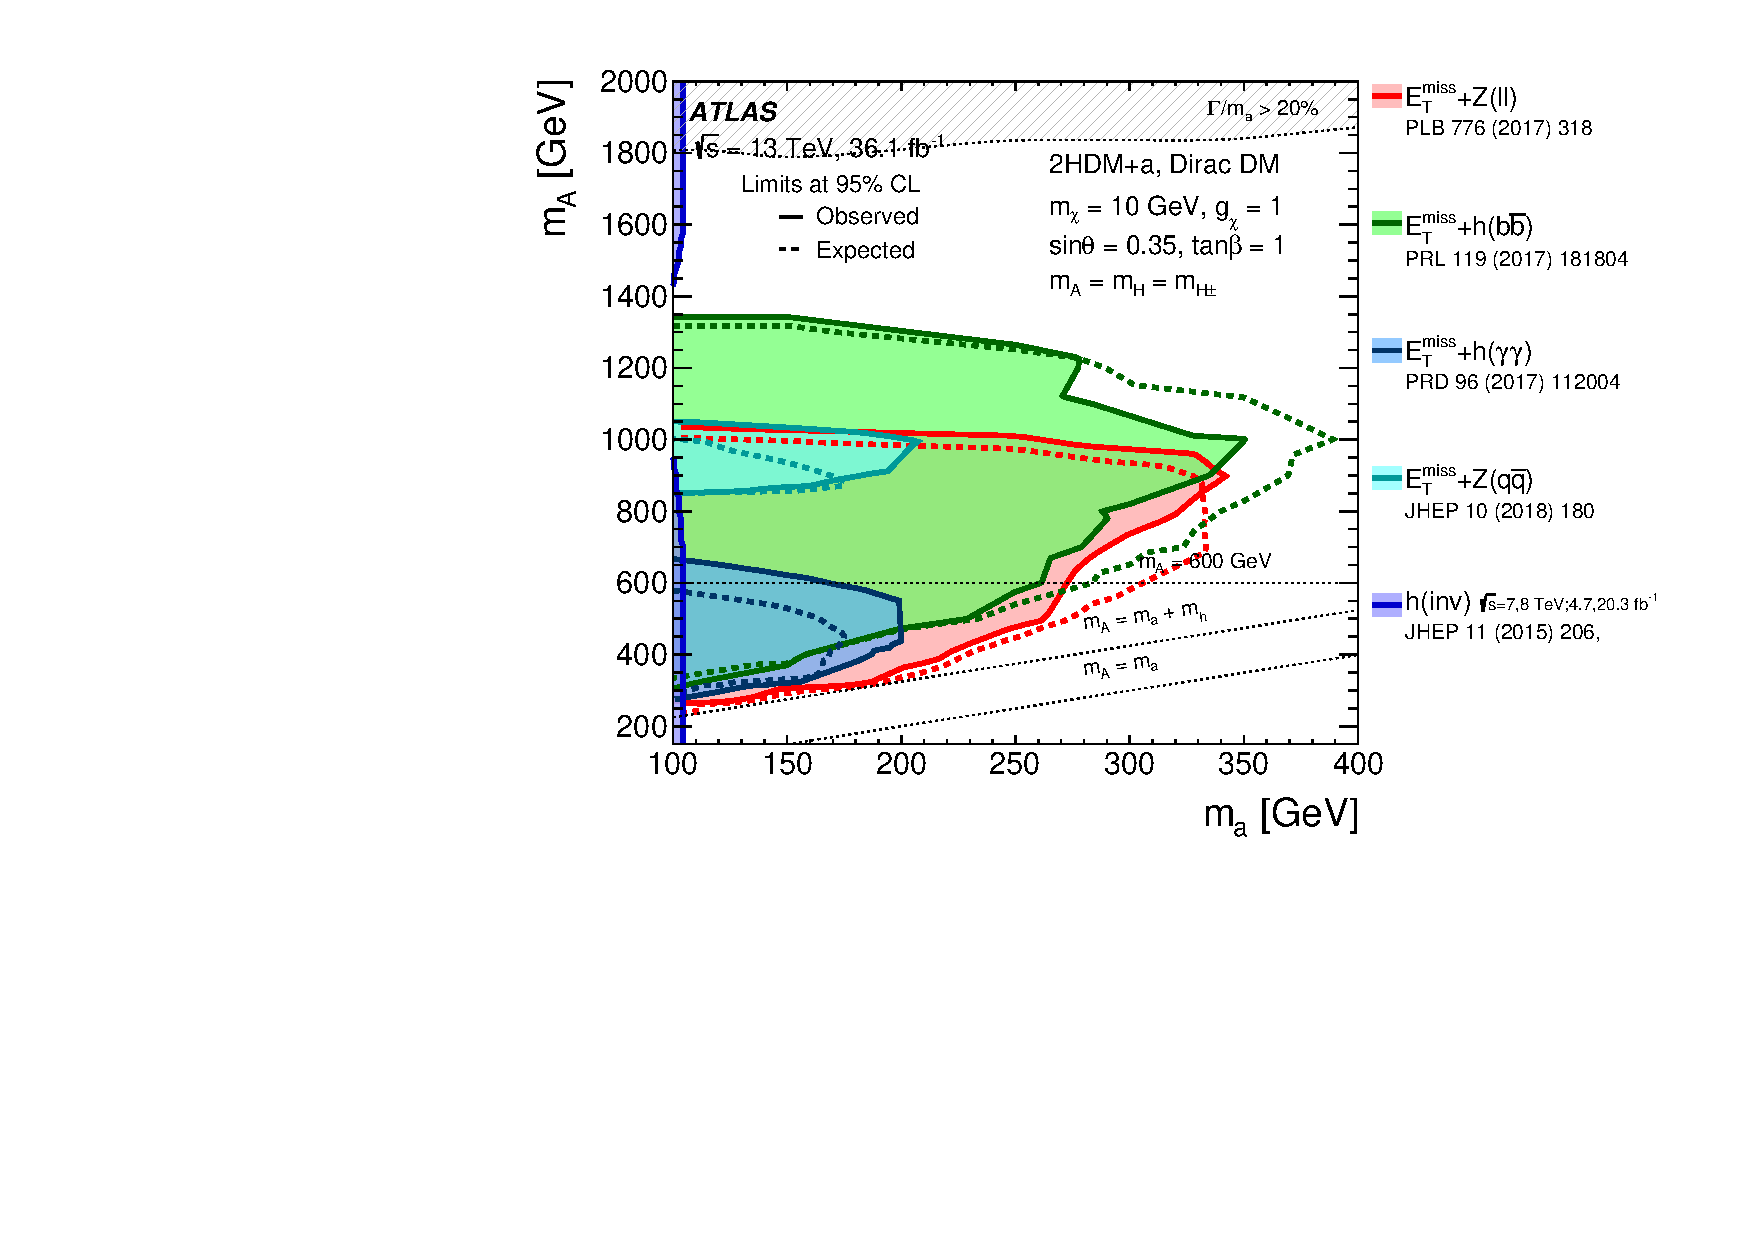
\includegraphics[width=1.\textwidth]{figures/outlook/ahdm/fig_19a.pdf}
    \caption{Exclusion contours at \SI{95}{\percent} \(\text{CL}_{s}\) for the \ahdm simplified model in the two-dimensional \mHiggsHeavy-\ma plane for the fixed choice of parameters \(\tan{\beta} = 1.0\), \(\mchi = \SI{10}{\giga\electronvolt}\), and \(\sin \theta = 0.35\), due to various \(\met + X\) searches and searches for invisible decays of the Higgs boson (\(\PHiggs + \text{invisible}\)). The dashed grey regions at the top indicate the region where the width of any of the Higgs bosons exceeds \SI{20}{\percent} of its mass. Figure reproduced from Ref.~\cite{EXOT-2017-32}.}
    \label{fig:outlook:higgs:ahdm-mHma}
\end{figure}

In addition to the \(\met + \HepProcess{Z(\Pq\Pq)}\) contour, the limits placed by the \(\met + \HepProcess{Z(\Pl\Pl)}\) search~\cite{HIGG-2016-28}, the \(\met + \Hbb\) search~\cite{EXOT-2016-25}, the \(\met + \HepProcess{\PHiggs \to \Pgg \Pgg}\) search~\cite{HIGG-2016-18}, the \(\met + \HepProcess{\Pqt \Paqt}\) search~\cite{SUSY-2016-18}, and searches for invisible decays of the Higgs boson (\(\PHiggs + \text{invisible}\))~\cite{HIGG-2015-03} are displayed. The exclusion sensitivity is vastly dominated by the \(\met + \HepProcess{Z(\Pl\Pl)}\) and \(\met + \Hbb\) searches. In contrast to the \(V/A\) simplified model, the most relevant signal processes involve the resonant production of \PZ and Higgs bosons, therefore the experimentally much cleaner \(\met + \PZ(\Pl\Pl)\) signature provides better sensitivity than the \(\met + \PZ(\Pq\Pq)\) signature.

\Cref{fig:outlook:higgs:ahdm-sintheta} shows the exclusion limits on the signal strength \(\mu\) for the \ahdm simplified model as a function of \(\sin{\theta}\) for the fixed parameter choices \(\tan{\beta} = 1.0\), \(\mchi = \SI{10}{\giga\electronvolt}\), considering a low-mass scenario with \(\mHiggsHeavy = \SI{600}{\giga\electronvolt}\), \(\ma = \SI{200}{\giga\electronvolt}\), and a high-mass scenario with  \(\mHiggsHeavy = \SI{1000}{\giga\electronvolt}\), \(\ma = \SI{350}{\giga\electronvolt}\).

\begin{figure}[htbp]
    \centering
    \begin{subfigure}{1.\textwidth}
      \centering
      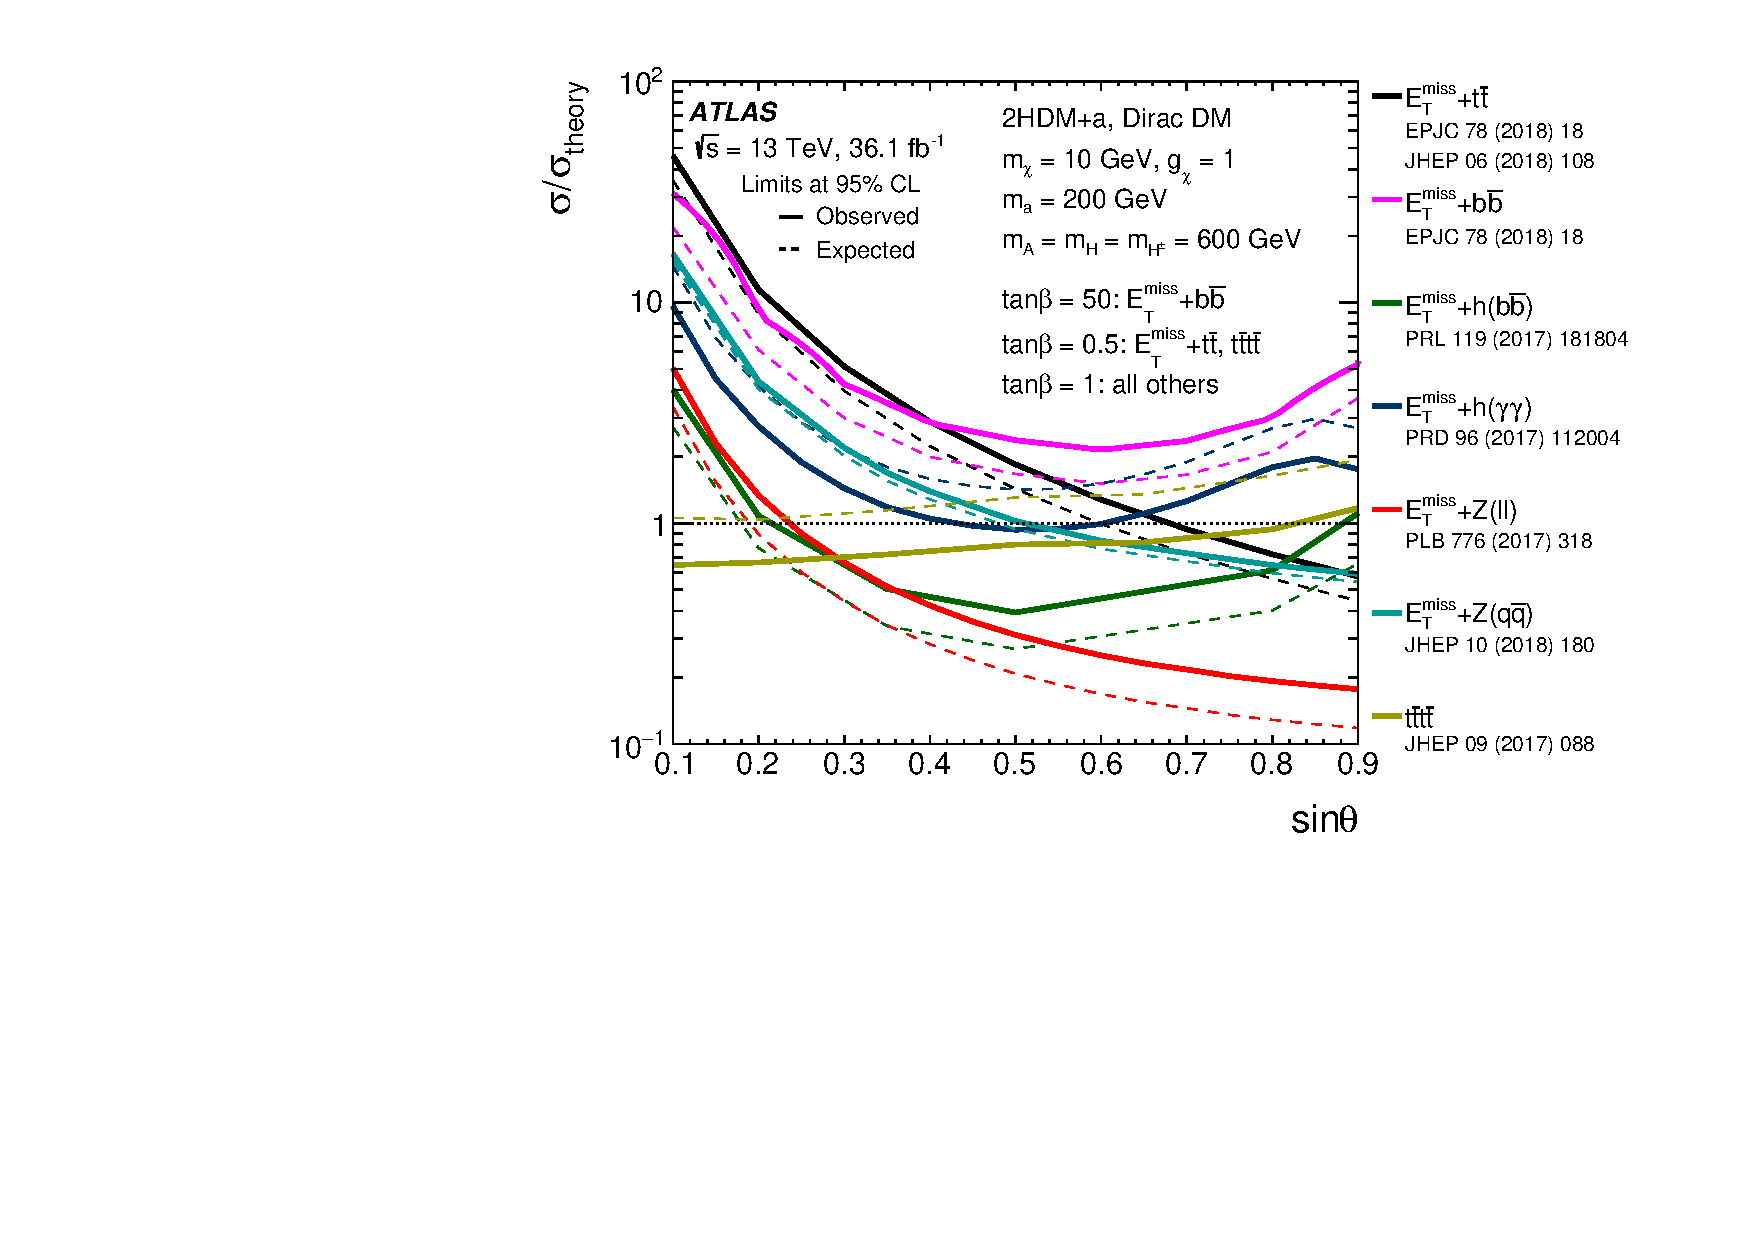
\includegraphics[width=.95\textwidth]{figures/outlook/ahdm/fig_20a.pdf}
      \caption{Low-mass scenario \(\mHiggsHeavy = \SI{600}{\giga\electronvolt}\), \(\ma = \SI{200}{\giga\electronvolt}\)}
    \end{subfigure}
    \\
    \begin{subfigure}{1.\textwidth}
      \centering
      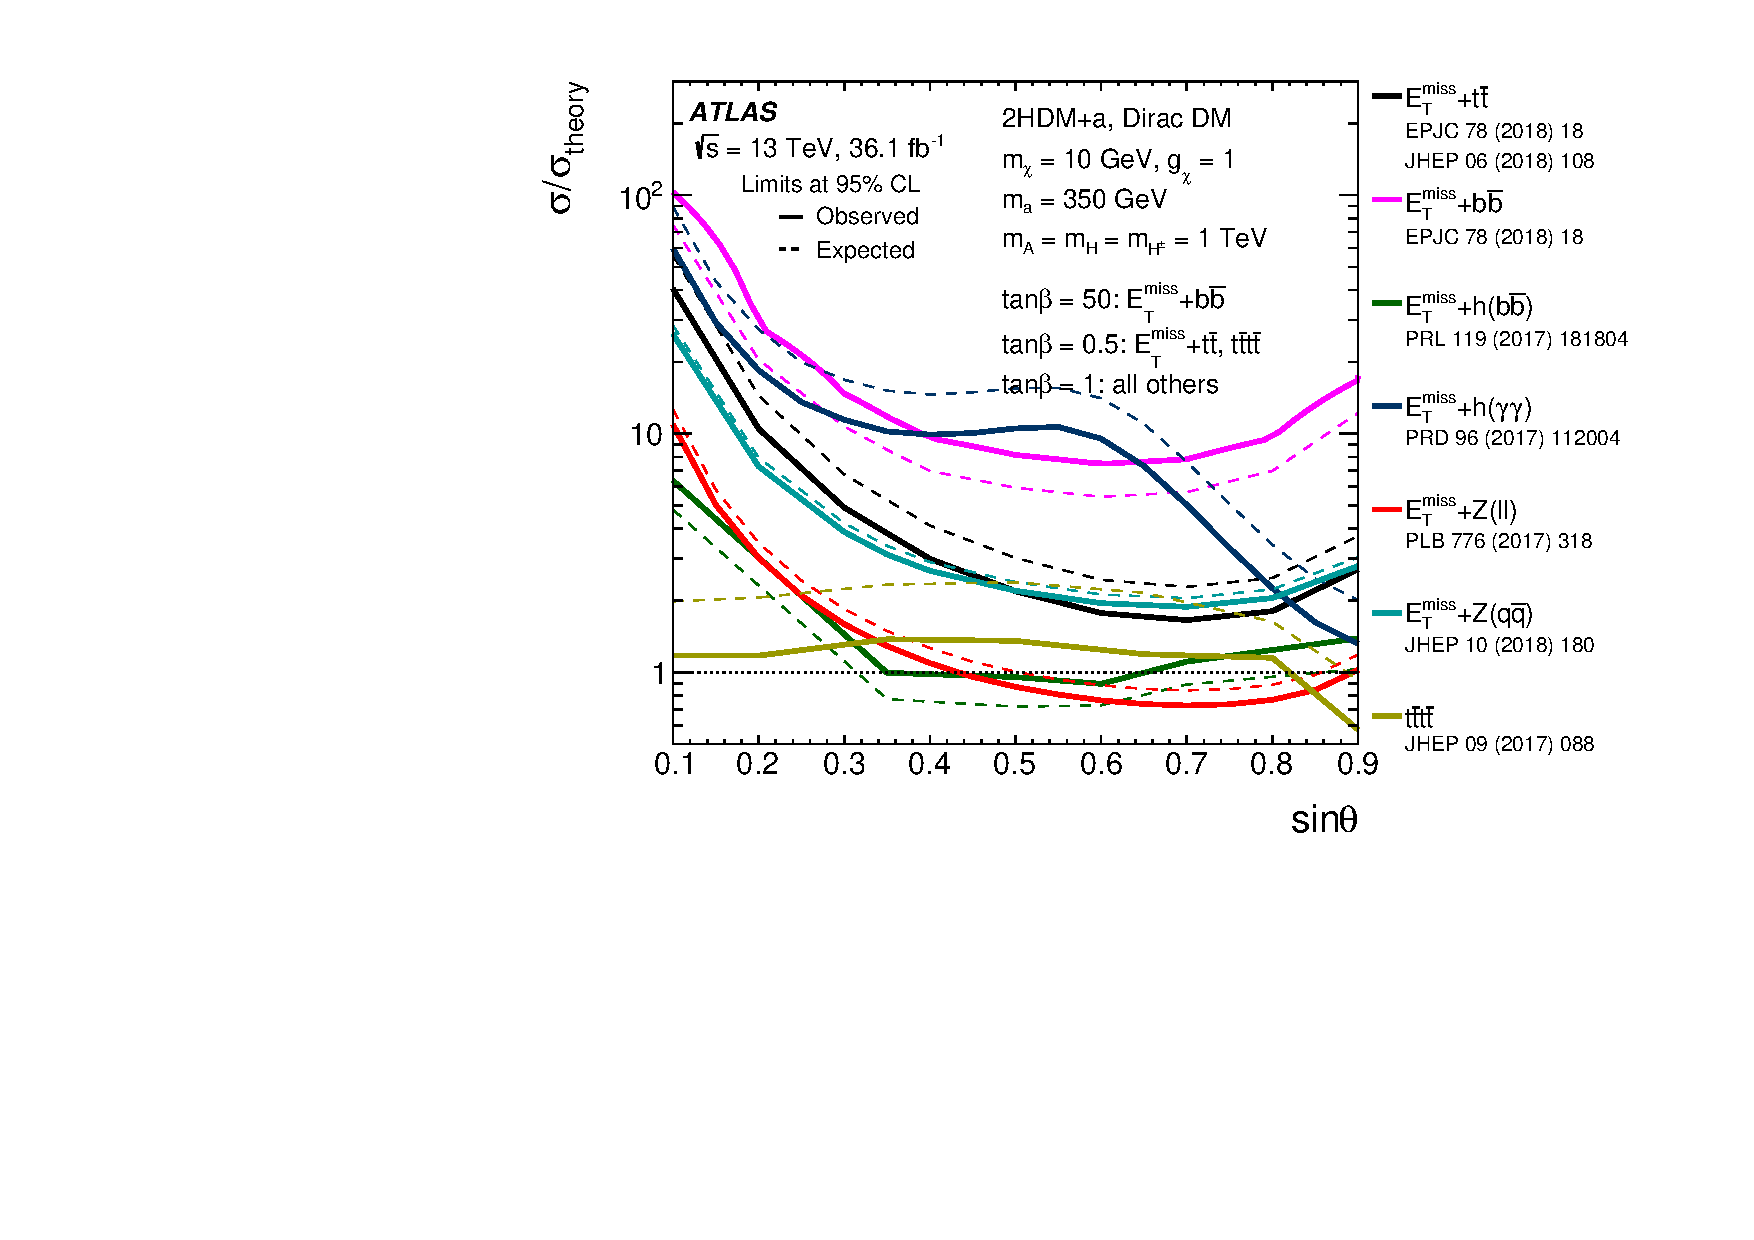
\includegraphics[width=.95\textwidth]{figures/outlook/ahdm/fig_20b.pdf}
      \caption{High-mass scenario \(\mHiggsHeavy = \SI{1000}{\giga\electronvolt}\), \(\ma = \SI{350}{\giga\electronvolt}\)}
    \end{subfigure}
    \caption{Observed exclusion limits at \SI{95}{\percent} \(\text{CL}_{s}\) on the signal strength \(\mu\) for the \ahdm simplified model as a function of \(\sin{\theta}\), shown for parameters corresponding to a low-mass scenario (top) and a high-mass scenario (bottom). Figures reproduced from Ref.~\cite{EXOT-2017-32}.}
    \label{fig:outlook:higgs:ahdm-sintheta}
\end{figure}

The strongest exclusion again is provided by the \(\met + \PZ(\Pl\Pl)\) and \(\met + \Hbb\) searches. While the sensitivity of the \(\met + \PZ\) searches improves monotonically as a function of \(\sin \theta\), the sensitivity of the \(\met + \Ph\) searches varies due to the non-trivial dependence of the Higgs boson \pt distribution on the mixing angle. The heavy-flavour signatures are presented for the different parameter choices \(\tan{\beta} = 0.5\) (\(\met + \ttbar\), \ttbar\ttbar) and \(\tan{\beta} = 50\) (\(\met + \bbbar\)), which result in enhanced coupling of the pseudo-scalar mediator to up-type or down-type quarks, respectively.

\Cref{fig:outlook:higgs:ahdm-mchi} shows the exclusion limits on the dark matter mass \mchi for the fixed choices of the parameters \(\tan{\beta} = 1.0\), \(\mHiggsHeavy = \SI{600}{\giga\electronvolt}\), \(\ma = \SI{250}{\giga\electronvolt}\), and \(\sin \theta = 0.35\). The dark matter mass is the parameter with the strongest impact on the relic density \(\Omega h^2\), which is overlaid as a blue long-dashed curve.

\begin{figure}[htbp]
    \centering
    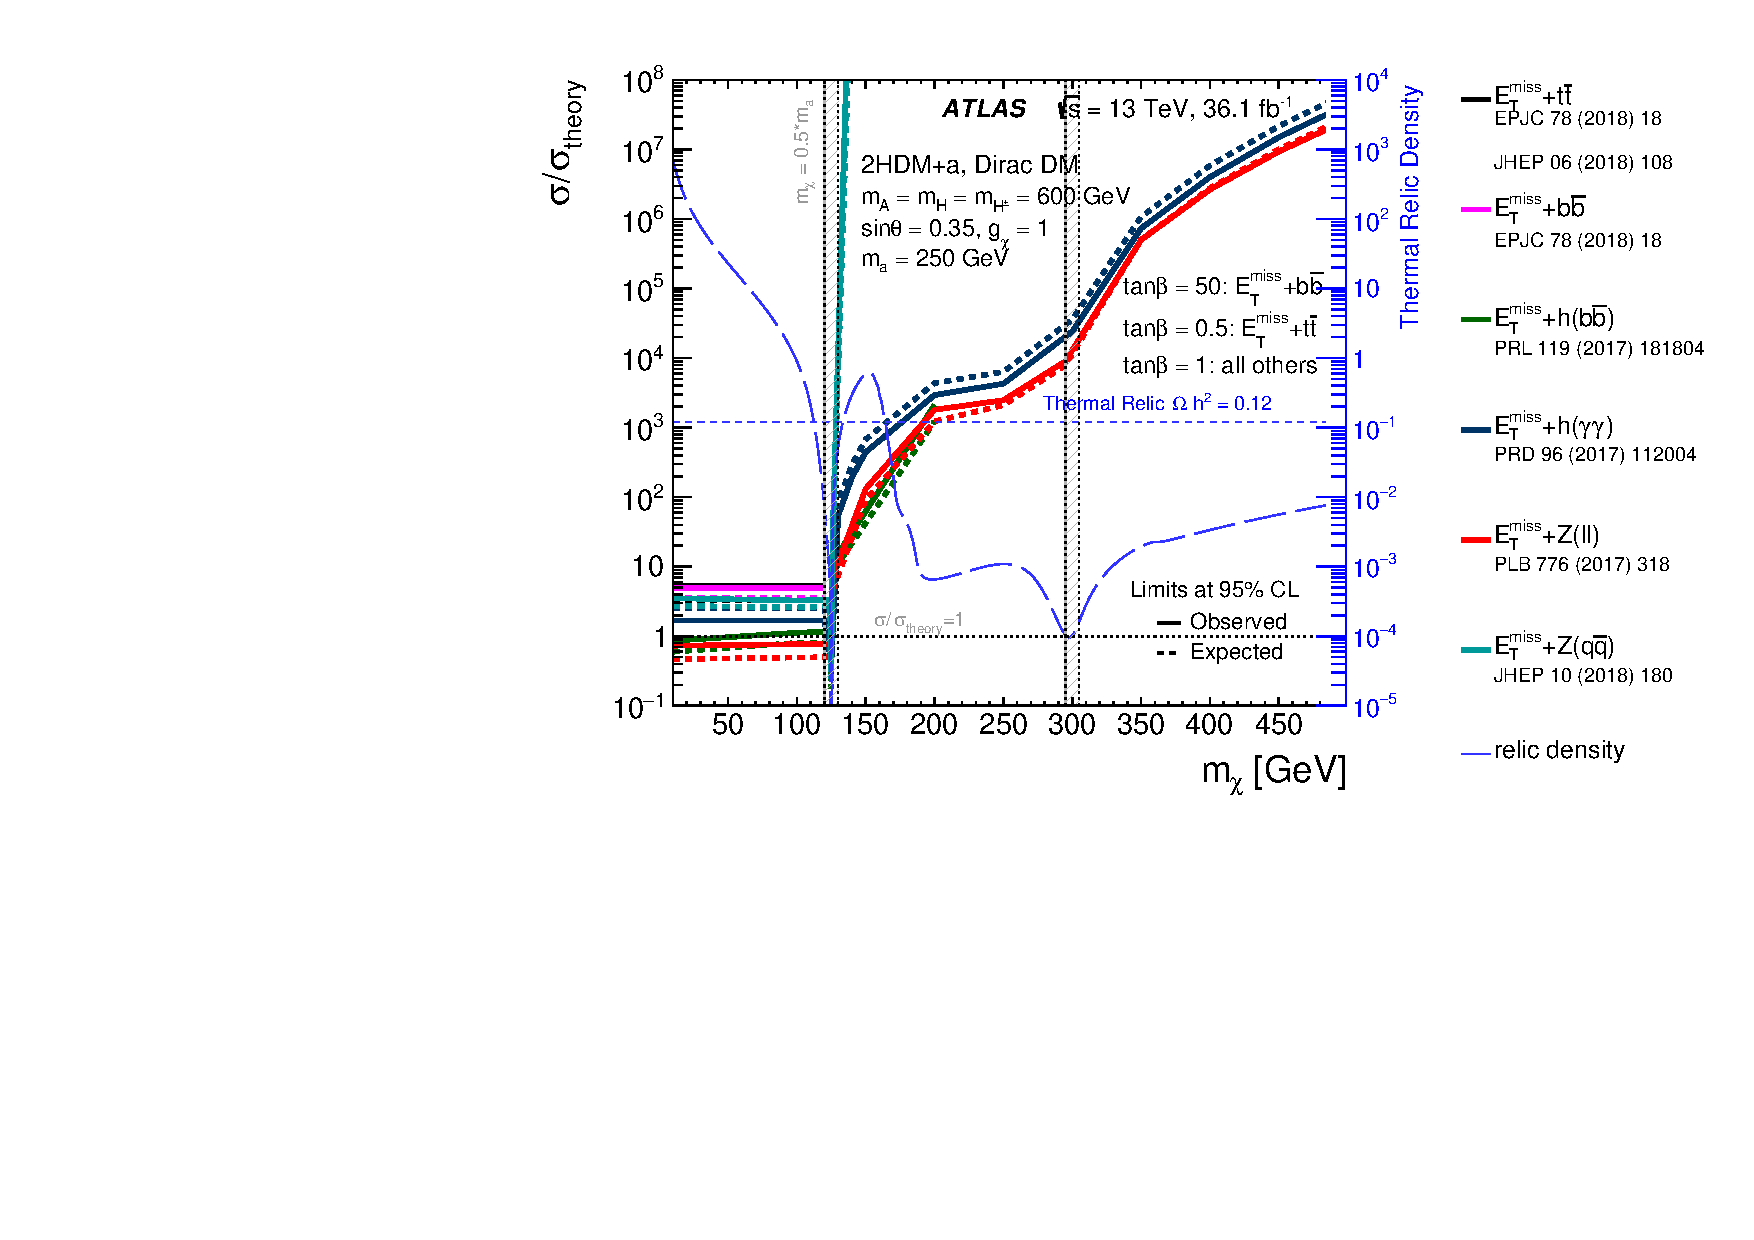
\includegraphics[width=1.0\textwidth]{figures/outlook/ahdm/fig_21.pdf}
    \caption{Exclusion limits at \SI{95}{\percent} \(\text{CL}_{s}\) on the signal strength \(\mu\) for the \ahdm simplified model as a function of \mchi for the fixed choices of the parameters \(\tan{\beta} = 1.0\), \(\mHiggsHeavy = \SI{600}{\giga\electronvolt}\), \(\ma = \SI{250}{\giga\electronvolt}\), and \(\sin \theta = 0.35\). The relic density prediction by the \ahdm simplified model is superimposed (long-dashed line). Figure reproduced from Ref.~\cite{EXOT-2017-32}.}
    \label{fig:outlook:higgs:ahdm-mchi}
\end{figure}

For dark matter masses close to \(\ma / 2\) or \(\mchi > \SI{170}{\giga\electronvolt}\), the predicted value of the relic density is equal to or below the observed value from Planck~\cite{Planck2020} measurements.
The sensitivity of all \(\met + X\) signatures under consideration is independent of \mchi in the on-shell region \(2 \mchi < \ma\). The \(\met + \PZ(\Pl\Pl)\) search excludes this parameter space. The sensitivity of these searches is resonantly enhanced close to the threshold \(\mchi = \ma / 2 = \SI{125}{\giga\electronvolt}\). For higher dark matter masses, the sensitivity strongly decreases, leaving the parameter choices for \(\mchi > \ma / 2\) which are not in conflict with the relic density measurements unconstrained.

The \ahdm simplified model is probed by several ATLAS dark matter searches~\cite{EXOT-2017-32,ATLAS-CONF-2020-034}. As it is the benchmark next-generation spin-0 dark matter model by the LHC DM WG~\cite{Abe2020}, its investigation is central to the ATLAS full Run-2 dark matter research programme.

\section{Simplified models with two mediators}
\label{sec:outlook:2mdm}
The simplified model containing both a spin-1 \PZprime and a spin-0 dark Higgs boson mediator extends the elementary simplified models in complexity by explicitly describing elements of their potential UV-completion. Consequentially, the model predicts additional signatures which were not considered in searches motivated by elementary simplified models.
One such neglected signature is the resonant production of a dark Higgs boson of unknown mass \ms in association with dark matter particles, which manifest as missing transverse momentum and result in boosted dark Higgs boson candidates. The dark Higgs boson hypothesis can be probed in different final states, depending on the branching fraction of the dark Higgs boson decays (c.f. \Cref{fig:dm:models:2mdm:darkhiggsbranching}) which is contingent on \ms.

\Cref{fig:outlook:2mdm:summary} shows the \SI{95}{\percent} \(\text{CL}_{s}\) on the signal strength \(\mu\) for the 2MDM simplified model as a function of \ms for the fixed choices of the parameters \(\mZp = \SI{1}{\tera\electronvolt}\), \(\mchi = \SI{200}{\giga\electronvolt}\), \(\gq = 0.25\), \(\gchi = 1\), and \(\theta = 0.01\).

\begin{figure}[htbp]
    \centering
    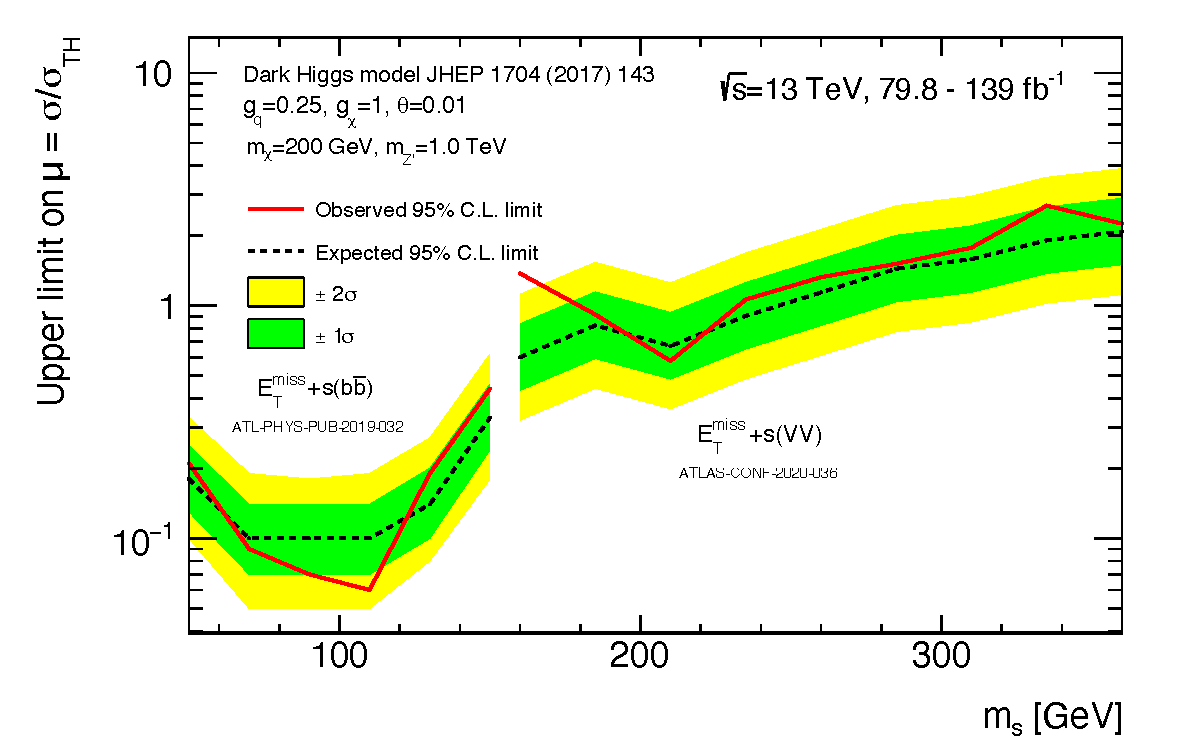
\includegraphics[width=0.85\textwidth]{figures/outlook/2mdm/monoSlimits_mZp1p0_summary.pdf}
    \caption{Exclusion limits at \SI{95}{\percent} \(\text{CL}_{s}\) on the signal strength \(\mu\) for the 2MDM simplified model as a function of \ms for the fixed choices of the parameters \(\mZp = \SI{1}{\tera\electronvolt}\), \(\mchi = \SI{200}{\giga\electronvolt}\), \(\gq = 0.25\), \(\gchi = 1\), and \(\theta = 0.01\).}
    \label{fig:outlook:2mdm:summary}
\end{figure}

For low \ms, the \(\met + \sbb\) search places stringent limits on the signal strength \(\mu\). For heavier \ms, the \(\met + \sVV\) search is able to probe the parameter space. The mild excess at \(\ms = \SI{160}{\giga\electronvolt}\) which is observed by the \(\met + \sVV\) search invites corroboration by further investigation of the \(\met + \sbb\) final state or by searches targeting the semi-leptonic \(\met + \sVV\) signature.

In summary, the 2MDM simplified model can avoid constraints from perturbative unitarity considerations, dark matter relic density measurements, and from direct detection experiments, thereby leading towards previously neglected signatures. Interestingly, the 2MDM simplified model also predicts \(\met + \PZprime\) signatures if the dark Higgs boson decays into invisible states and the \PZprime boson decays hadronically, which are probed in similar final states as those considered in the \(\met + \Vqq\) search~\cite{EXOT-2016-23,Gadow2018}. Further exploration of this model's viable parameter space by a combination of searches in different final states seems promising.
